\documentclass[tikz,border=10pt]{standalone}
\usetikzlibrary{shapes}
\usetikzlibrary{arrows}
\usetikzlibrary{positioning}
\begin{document} 
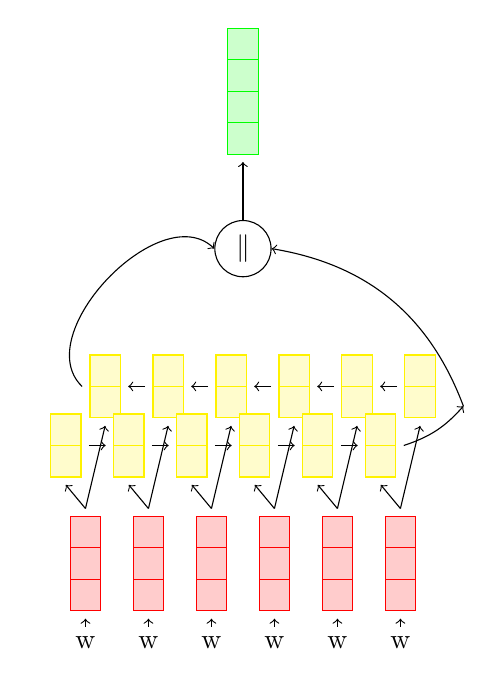
\begin{tikzpicture}[
  hid/.style 2 args={
    rectangle split,
    draw=#2,
    rectangle split parts=#1,
    fill=#2!20,
    outer sep=1mm}]

 \foreach \i [count=\step from 1] in {w, w, w, w, w, w}
    \node (i\step) at (.8*\step, -2) {\i};
  % draw embedding and hidden layers for text input
  \foreach \step in {1,...,6} {
    \node[hid={3}{red}] (e\step) at (.8*\step, -1) {};    
    \draw[->] (i\step.north) -> (e\step.south);
  }

  \foreach \step in {1,...,6} {
    \node[hid={2}{yellow}] (h_f_\step) at (-.25 + .8 *\step, .5) {};    
    \node[hid={2}{yellow}] (h_r_\step) at (.25 + .8 *\step, 1.25) {};    
    \draw[->] (e\step.north) -> (h_f_\step.south);
    \draw[->] (e\step.north) -> (h_r_\step.south);
  }
 % \foreach[count=\i, evaluate=\i as \x using int(\i+9)] \step in {8,...,10} {
  \foreach \step/\steppp in {1/2, 2/3, 3/4, 4/5, 5/6} {
   
    \draw[->] (h_f_\step.east) -> (h_f_\steppp.west);
    \draw[->] (h_r_\steppp.west) -> (h_r_\step.east);
  }
 
\node[circle,draw=black] (concat) at (3 * .8 + .4, 3) {$\Vert$};
\coordinate (g) at (7 * .8, 1);
\path[->] (h_r_1.west) edge[bend left=90] (concat.west);
\path[->] (h_f_6.east) edge[bend right=15] (g) 
          (g) edge[bend right] (concat.east);
\node[hid={4}{green}] (s2) at (3 * .8 + .4, 5) {};
\path[->] (concat) edge (s2);
 


\end{tikzpicture}
\end{document}
